\chapter{Hash}
\section{Dizionari}
I dizionari sono strutture dati fondamentali che consentono di rappresentare una relazione tra
un insieme di chiavi D, il dominio, e un insieme di valori C, il codominio. Questa associazione
chiave-valore è comunemente utilizzata in diverse applicazioni come le rubriche telefoniche, dove
ogni numero di telefono (chiave) è associato a un nome (valore). Le operazioni principali che
devono essere supportate efficientemente da un dizionario sono:
\begin{itemize}
    \item \textbf{Insert:} aggiunge un nuovo valore
    \item \textbf{Search:} restituisce il valore associato a una chiave
    \item \textbf{Delete:} elimina un valore dalla struttura
\end{itemize}
\noindent Esistono diversi modi per implementare un dizionario, tra cui:
\begin{itemize}
    \item tebelle ad indirizzamento diretto
    \item tabelle di hash
\end{itemize}
\section{Tabelle ad indirizzamento diretto}
L’indirizzamento diretto è una tecnica efficace quando U, l’universo delle chiavi, è ragionevolmente
 piccolo, ovvero dato $U= {0, 1, ..., m-1}$, con $m$ non troppo grande. Le tabelle ad
indirizzamento diretto utilizzano un array per gestire le chiavi e rappresentare l’insieme dinamico 
in cui ogni elemento ha associata una chiave estratta dall’universo $U$. Supponendo che due
elementi non possano avere la stessa chiave, si può rappresentare l’insieme dinamico utilizzando
un array o tavola a indirizzamento diretto indicata con $T[0 ...m-1]$, dove ogni posizione
o cella dell’array è associata a una chiave specifica, e il valore associato ad essa è memorizzato
nell’array. La cella $k$ punta a un elemento dell’insieme con chiave $k$. Se nessun elemento è
associato ad una specifica chiave $k$, allora $T[k] = NIL$.
\begin{figure}[H]
    \centering  
    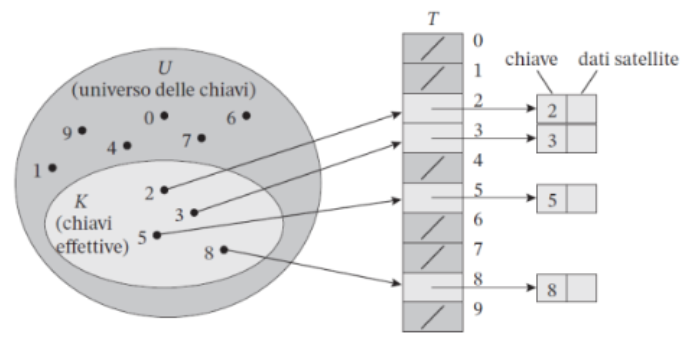
\includegraphics[width=0.5\linewidth]{../images/tabelle_indirizzamento_diretto.png}
    \label{label}
\end{figure}
\subsection{Operazioni su una tabella ad indirizzamento diretto} 
Le operazioni su una tabella ad indirizzamento diretto sono le seguenti:
\begin{itemize}
    \item \textbf{Search(T, k):} restituisce $T[k]$;
    \item \textbf{Insert(T, x):} imposta $T[x.key]=x$;
    \item \textbf{Delete(T, x):} imposta $T[x.key]=nil$
\end{itemize}
\textbf{Analisi}\\
I principali \textbf{vantaggi} delle tabelle a indirizzamento diretto includono operazioni di inserimento,
ricerca e cancellazione molto efficienti in tempo $O(1)$.\\
Bisogna notare quanto sia vantaggiosa la possibilit`a di evitare di memorizzare la chiave e i
dati satelliti di un elemento in un oggetto esterno puntato da una cella dell’array $T$, al contrario
è possibile memorizzare l’oggetto nella cella stessa, risparmiando spazio e usando l’indice come
chiave.\\
Tuttavia, presentano anche significativi \textbf{svantaggi}, infatti con l’indirizzamento diretto si è
”costretti” ad allocare memoria per una tabella $T$ di dimensione $|U|$, ovvero pari alla cardinalità
dell’insieme dell’universo delle chiavi. Se l’universo è troppo grande può essere impraticabile
allocare così tanta memoria, inoltre potrebbe succedere che l’insieme $K$ delle chiavi effettivamente 
memorizzate sia così piccolo rispetto a $U$ che la maggior parte dello spazio allocato per
la tabella $T$ sarebbe sprecato.
\subsection{Fattore di carico}
Il fattore di carica $\alpha$ misura il grado di riempimento di una tabella ed è definito come $\alpha= n/m$
dove $n = |K|$ è il numero di chiavi effettivamente utilizzate e $m = |U|$ la dimensione della
tabella.

\section{Tabelle o tavole di Hash}
Le tabelle hash rappresentano un’evoluzione delle tabelle ad indirizzamento diretto, utilizzando
una funzione di hash per mappare le chiavi alle posizioni dell’array. Se con l’indirizzamento
diretto un elemento con chiave $k$ è memorizzato nella cella $k$, con l’hashing, questo elemento
è memorizzato nella cella $h(k)$, ovvero si utilizza una funzione di hash $h$ per calcolare la cella
della chiave $k$. Dunque la funzione \textbf{h} associa ogni chiave $k$ a una posizione $h(k)$ nell’array.
\begin{figure}[H]
    \centering  
    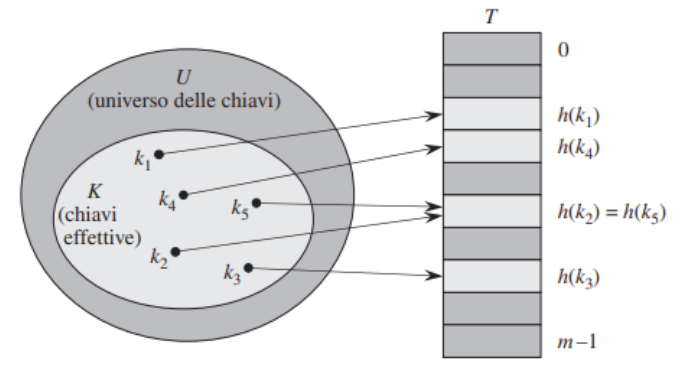
\includegraphics[width=0.5\linewidth]{../images/tabella-hash.png}
    \label{label}
\end{figure}
\noindent La funzione hash $h: U \rightarrow {0,..,m-1}$ associa l’universo U delle possibili chiavi alle 
celle di una tabella di hash $T[0 ...m-1]$ dove la dimensione m della tabella è generalmente più piccola
di $|U|$, in questo modo la dimensione dell’array viene ridotta e sarà proporzionale al numero
massimo di chiavi presenti nel dizionario.
\subsection{Collisioni}
Tuttavia, essendo $|U|>m$, si verificano collisioni quando due chiavi diverse, $k_1 \neq k_2$, vengono mappate alla stessa posizione $h(k_1)=h(k_2)$.\medskip\\
\textbf{Il principio della PICCIONAIA}\\
Se p piccioni devono trovare posto in c caselle e ci sono più piccioni che caselle allora
in qualche casella entreranno almeno due piccioni.\medskip\\
\textbf{Gestione delle collisioni}\\
La gestione delle collisioni è cruciale per l'efficienza delle tabelle hash. Esistono due metodi principali:
\begin{itemize}
    \item Metodo del concatenamento
    \item Metodo dell'indirizzamento aperto
\end{itemize}

\subsection{Metodo del concatenamento (Liste di trabocco)}
\begin{figure}[H]
    \centering  
    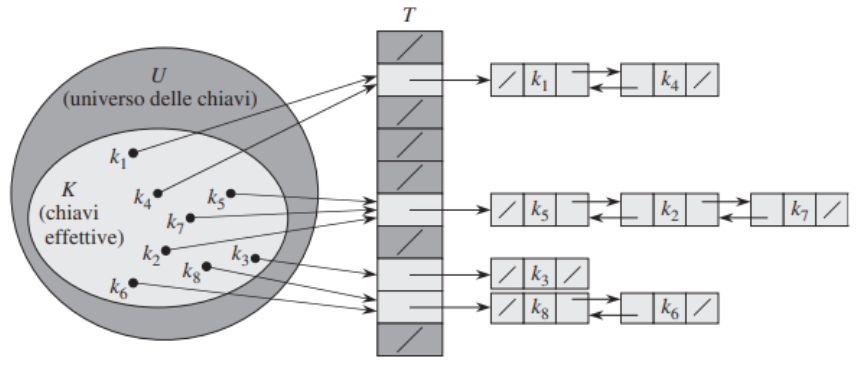
\includegraphics[width=0.5\linewidth]{../images/metodo-concatenamento.png}
    \label{label}
\end{figure}
\noindent L’insieme di input di $n$ elementi viene diviso casualmente in $m$ sottoinsiemi, ciascuno di cardinalità 
$n/m$. Una funzione di hash determina a quale sottoinsieme appartiene un elemento,
ovvero associa ad ogni elemento una chiave, per gestire i vari sottoinsiemi (chiavi) si realizzano
delle liste collegate. Immaginiamo di avere più chiavi $k1  \neq k2  \neq k3$ mappate su una stessa
cella $j$ dell’array $T$, questa ha un puntatore alla testa della lista concatenata che conterrà tutti
gli elementi memorizzati in $j$, se non ci sono elementi, la cella $j$ contiene la costante $NIL$. Per
concatenare le liste associate a chiavi mappate alla stessa posizione si usufruisce di un doppio
puntatore.

\subsection{Operazioni sulle liste di trabocco}
Le operazioni su una tabella con liste di trabocco sono le seguenti:
\begin{itemize}
    \item \textbf{Search(T,k):} cerca nella lista $T[h(k)]$ un elemento $x$ tale che $x.key==k$ e lo restituisce
    \item \textbf{Insert(T,x):} aggiunge $x$ nella lista $T[h(x.key)]$
    \item \textbf{Delete(T,x):} toglie $x$ dalla lista $T[h(x.key)]$
\end{itemize}

\subsection{Fattore di carico}
Il concetto di fattore di carico $\alpha$ per il metodo del concatenamento può essere ridefinito come
segue: data una tavola hash $T$ con $m$ celle dove sono memorizzati $n$ elementi, si definisce fattore
di carico $\alpha$ come il rapporto $n/m$, ossia il numero medio di elementi memorizzati in una
lista.

\subsection{Analisi}
L’analisi sarà fatta in funzione del fattore di carico $\alpha$, che può essere minore, uguale o maggiore
di $1$. Il caso peggiore si presenta quando tutte le n chiavi sono associate alla stessa cella, così
creando una lista di lunghezza $n$ con operazioni che richiedono il seguente tempo di esecuzione:
\begin{itemize}
    \item \textbf{Search(T,k):} \textbf{$\Theta(n)$} $+$ tempo di calcolo della funzione di hash 
    \item \textbf{Insert(T,x):} \textbf{$O(1)$} con l'assunzione che $x$ non sia già nel dizionario, se questa assunzione non valore
    allora si paga il costo di una precedente search
    \item \textbf{Delete(T,x):} \textbf{$O(1)$} se le liste sono doppiamente concatenate, ovvero quando ogni nodo
della lista ha un campo $next$ che punta al nodo successivo e un campo $prev$ che punta al
nodo precedente, altrimenti il costo di una search 
\end{itemize}
\noindent Le prestazioni dell’hashing nel caso medio dipendono dal modo in cui la funzione hash h 
distribuisce l’insieme delle chiavi da memorizzare tra le $m$ celle.\\
Supponiamo che qualsiasi elemento abbia la stessa probabilità di essere mandato in una qualsiasi delle $m$ celle, indipendentemente
dalle celle in cui sono mandati gli altri elementi, si tratta così l’ipotesi di \textbf{hash uniforme indipendente}.
\subsection{Teoremi metodo del concatenamento}
\textbf{Teorema 1}
\begin{theorem}
In una tabella hash le cui collisioni sono risolte tramite la tecnica del concatenamento, una
ricerca senza successo richiede in media un tempo $\Theta(1 + \alpha)$, nell’ipotesi di hashing
uniforme e indipendente.
\end{theorem}
\noindent \textbf{Teorema 2}
\begin{theorem}
In una tabella hash le cui collisioni sono risolte tramite la tecnica del concatenamento, una
ricerca con successo richiede in media un tempo $\Theta(1 + \alpha)$, nell’ipotesi di hashing
uniforme e indipendente.
\end{theorem}
\noindent \textbf{Corollario}
\begin{corollario}
    Utilizzando l'hashing universale e risolvendo le collisioni tramite concatenamento in una 
    tabella inizialmente vuota di m celle, il tempo atteso per gestire qualsiasi sequenza di s 
    operazioni Insert, Search e Delete contenente $n=O(m)$ operazioni INSERT è $\Theta(s)$
\end{corollario}
\subsection{Funzioni di hash}
\begin{figure}[H]
    \centering  
    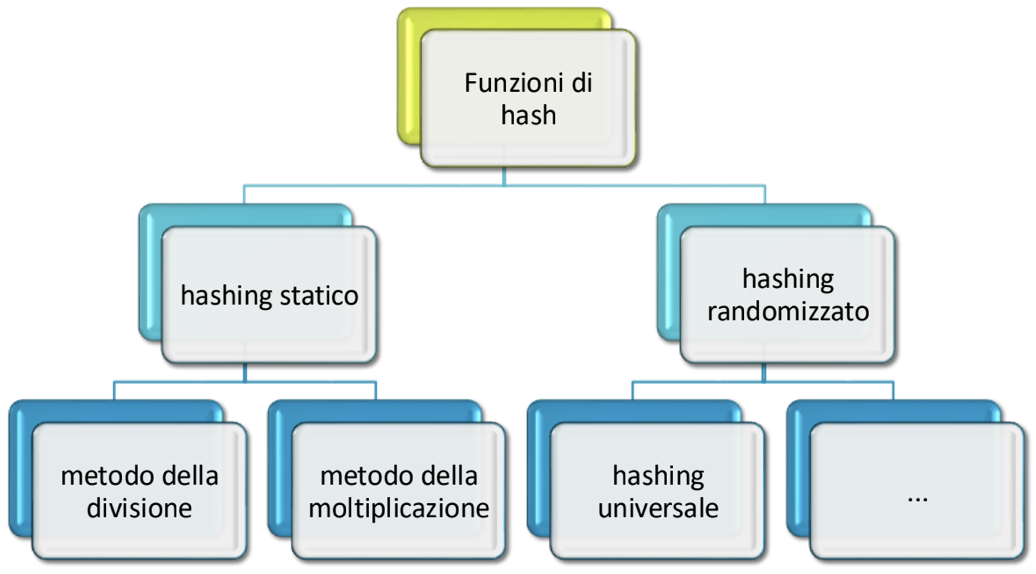
\includegraphics[width=0.5\linewidth]{../images/funzioni-hash.png}
    \label{label}
\end{figure}
Esistono degli schemi per poter progettare e realizzare delle buone funzioni di hash, due sono
di tipo euristico, ovvero l’hashing per divisione e quello per moltiplicazione, mentre il terzo
usa la randomizzazione ed è denominato hashing universale. Una buona funzione di hash
soddisfa l’ipotesi dell’hashing uniforme indipendente: ogni chiave ha la stessa probabilità
$1/m$ di essere mandata in una qualsiasi delle $m$ celle, indipendentemente dalle chiavi inserite
precedentemente.\\
Se le chiavi sono rappresentate da numeri reali $x$ estratti casualmente e indipendentemente
da una distribuzione di probabilità uniforme nell’intervallo $0 \le x < 1$, la funzione di hash
$h(x) = \lfloor m \cdot x \rfloor$ soddisfa l’ipotesi di hash uniforme indipendente.\\
Poiché questa ipotesi dipende dalle probabilità con cui vengono estratti gli elementi da inserire
e, questa probabilità in genere non è nota, si assume che l’universo delle chiavi sia l’insieme
dei numeri naturali interi non negativi. Questa assunzione non è restrittiva, in quanto ogni
tipo di chiave è rappresentato nel calcolatore con una sequenza di bit e ognuna di esse si può
interpretare come un intero non negativo.

\subsection{Hashing Statico}
\textbf{Metodo divisione}\\
Associa ad una chiave $k$ una delle $m$ celle prendendo il resto della divisioe intera tra $k$ e $m$, ovvero\\
$$h(k)=k \mod m$$\\
Per esempio, se la tavola hash ha dimensione $m = 12$ e la chiave è $k = 100$, allora
$h(k) = 4$. Quando si utilizza questo metodo vengono evitati certi valore di $m$, ad esempio
$m$ non dovrebbe essere una potenza di $2$, perchè se $m = 2 \cdot p$, allora $h(k)$ rappresenta
proprio i $p$ bit meno significativi di $k$. Una buona scelta per $m$ è un numero primo non
troppo vicino ad una potenza esatta di $2$. Ad esempio $m= 701$ perchè è un numero primo
vicino a $2000/3$, ma non a una potenza di $2$.\medskip\\
\textbf{Meotdo della moltiplicazione}\\
Questo metodo si svolge in due passi, prima moltiplica la chiave $k$ per una costante $A$ (comoresa tra 0 e 1) e si estrae la parte frazionaria di $k \cdot A$. 
Dopodiche si moltiplica il valore ottenuto per $m$ e prende la parte intera inferiore del risultato. La funzione di hash è\\
$$h(k)=\lfloor m(k A \mod 1) \rfloor$$\\
dove "$k \cdot A \mod 1$" rappresenta la parte frazionaria di $k \cdot A$, cioè $k \cdot A - \lfloor k \cdot A \rfloor$.
Un vantaggio del metodo della moltiplicazione è che il valore di $m$ non è critico.\\
Tipicamente, si sceglie $m$ pari ad una potenza di $2$ ($m=2^{p}$ per qualche intero $p$).\\
Supponiamo che ogni chiave $k$ possa essere rappresentata da una sola parola di $w$ bit.\\
Come $A$ prendiamo una frazione della forma $q/2^w $, dove quando $q$ è un intero nell'intervallo 
$0 < q < 2^w $. Prima si moltiplica $k$ per l'intero di $w$ bit $q=A \cdot 2^w $. Il risultato è un valore di 
$2 \cdot w$ bit $r_1 2^w + r_0$ dove $r_1$ è la parte più significativa del prodotto e $r_0$ è la parte 
meno significativa del prodotto. Il valore hash desiderato di $p$ bit è formato dai $p$ bit più significativi di $r_0$.\medskip\\
\begin{figure}[H]
    \centering  
    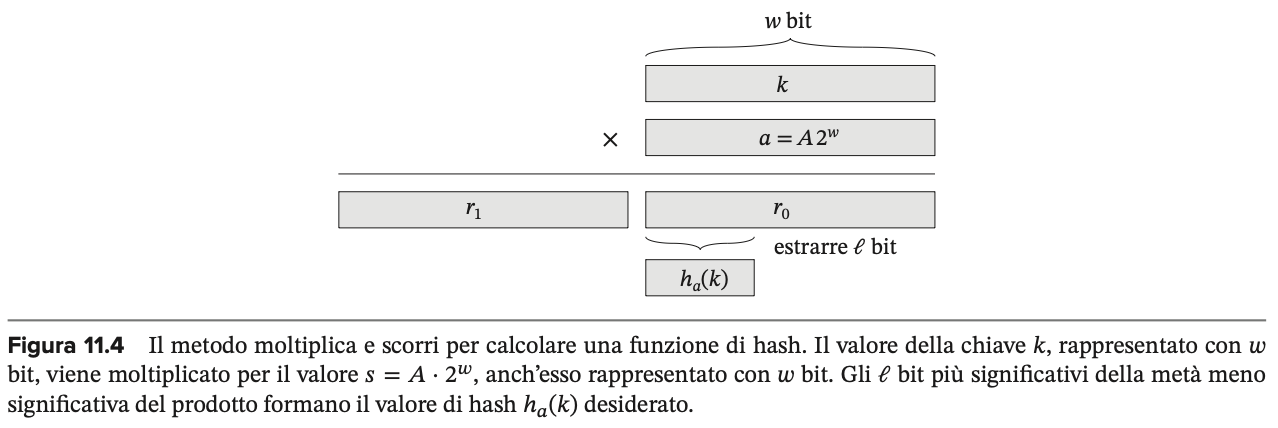
\includegraphics[width=0.75\linewidth]{../images/moltiplica_scorri_hash.png}
    \label{label}
\end{figure}
\noindent \textbf{Warning}\\
Nessuna funzione di hash può evitare che un avversario malevolo inserisca
nella tabella una sequenza di valori che vadano a finire tutti nella stessa lista\\
Più in generale, per ogni funzione di hash si possono trovare delle distribuzioni
di probabilità degli input per le quali la funzione non ripartisce bene le chiavi
tra le varie liste della tabella hash
\subsection{Hashing Randomizzato}
Possiamo usare la randomizzazione per rendere il comportamento della tabella hash indipendente dall'input.\\
L’idea è quella di usare una funzione di hash scelta casualmente in un insieme
“universale” di funzioni di hash.
Questo approccio viene detto \textbf{hashing universale}.\medskip\\
\textbf{Definizione Hashing Universale}
\begin{definition}
Un insieme $H$ di funzioni di hash che associano un dato universo U di chiavi nell'insieme ${0,1,..,m-1}$ degli indici della tabella 
hash si dice universale se, per ogni coppia di chiavi diverse $j$ e $k$ vi sono al più $|H|/m$ funzioni di hash in $H$ tali che 
$h(j)=h(k)$\\    
\end{definition}
\noindent In altre parole, con una funzione di hash scelta a caso da $H$, la probabilità di collisione fra
due chiavi distinte $j$ e $k$ non è maggiore della probabilità $1/m$ di una collisione nel caso in cui
$h(k)$ e $h(j)$ fossero scelte in modo casuale e indipendente dall’insieme degli indici della tabella
hash (hashing universale indipendente).

\subsection{Progettare una famiglia universale di funzioni di hash - Metodo basato sulla teoria dei numeri}
Iniziamo scegliendo un numero primo $p$ sufficientemente grande in modo che sia maggiore di
ogni possibile chiave $k$. Supponendo che la dimensione dell’universo delle chiavi sia maggiore
del numero di celle nella tavola hash, abbiamo $p>m$. Adesso definiamo la funzione hash $h_{a,b}$
per ogni coppia di interi $(a, b)$ tali che $1 \le a < p$ e $0 \le b < p$ come segue, ovvero utilizzando
una trasformazione lineare seguita da riduzioni modulo $p$ e poi modulo $m$:\\
$$h_{a,b}(k)=[(ak+b)\mod p] \mod m$$\\
La famiglia di tutte queste funzioni hash è\\
$$ H_{pm} = { h_{a,b}: 1 \le a < p, 0 \le b < p } $$\\
con $p$ numero primo, ed è universale.\medskip\\
\textbf{Teorema}
\begin{theorem}
    La famiglia di funzioni $H={h_a:a \text{ è dispari, }1<q<m}$ dove
    $h_a(k)=(ka \mod 2^W)$ ottenuta tramite metodo moltiplica e scorri è $2/m-universale$
\end{theorem}

\section{Metodo dell'indirizzamento aperto}
Nell’indirizzamento aperto, tutti gli elementi sono memorizzati nella tavola hash stessa, ovvero
ogni cella della tavola contiene un elemento dell’insieme dinamico o la costante $NIL$. Non si
utilizzano puntatori a zone esterne di memoria, motivo per il quale un inserimento potrebbe
non andare a buon fine a causa del fatto che la tabella potrebbe essere piena, perciò il fattore
di carica $\alpha$ non supera mai 1.
Per effettuare un inserimento si esaminano in successione le posizioni della tabella hash (ispezione), 
finché non si trova una cella vuota in cui inserire la chiave. Anziché seguire sempre lo
stesso ordine $0, 1, ..., m-1$, la sequenza delle posizioni esaminate durante un’ispezione dipende
dalla chiave da inserire. Per tal motivo, la funzione di hash è una funzione $h(k, i)$ che al variare
di $i$ tra $0$ e $m-1$ fornisce, per ciascuna chiave $k$, una sequenza di indici ${h(k,0), h(k,1), ..., h(k,m-1)}$ 
che rappresenta l’ordine di ispezione. Volendo poter ispezionare tutte le celle, la sequenza
deve essere una permutazione dell’insieme degli indici della tabella.\bigskip\\
\textbf{Ricorda:} nello pseudocodice di Insert si suppone che gli elementi della tavola hash $T$ siano chiavi senza dati satelliti, 
ovvero la chiave $k$ è identica all'elemento che contiene la chiave $k$.\\
Ogni cella contiene una chiave o la costante $NIL$ (se la cella è vuota).\bigskip\\
\textbf{Ricorda:} quando cancelliamo una chiave della cella $i$, non possiamo semplicemente 
marcare questa cella come vuota inserendovi la costante $NIL$. Così facendo, 
potrebbero essere interrotte le sequenze di ispezione. Una soluzione consiste nel marcare 
la cella registrandovi il valore speciale \textbf{DELETED}, anziché $NIL$. 
Di conseguenza è necessario adattare la funzione Insert.\bigskip\\
\textbf{Pseudcodice}
\begin{verbatim}
    Insert(T, k){
        i = 0
        while i != m
            j = h(k,i)
            if T[j] == nil or T[j] == DELETED
                T[j] = K
                return j
            else 
                i = i + 1
        return "tabella piena" 
    }

    Search(T, k){
        i = 0
        while i != m and T[q] != nil
            q = h(k,i)
            if T[q] == K
                return q
            i = i + 1
        return nil 
    }

    Delete(T, i){
        T[i] = DELETED
    }
\end{verbatim}
\noindent Con l'indirizzamento aperto, la funzione di hash fornisce una sequenza di ispezione, 
pertanto si modifica l'ipotesi di hashing indipendente e uniforme si parla di hashing con 
permutazioni indipendenti e uniformi. Per \textbf{l'hashing uniforme} si suppone che ogni chiave abbia la stessa 
probabilità $1/m!$ di generare una qualsiasi delle $m!$ possibili sequenze di ispezione.\\
Esistono tre tecniche comunemente utilizzate per calcolare le sequenze di ispezione richieste 
dall'indirizzamento aperto:
\begin{enumerate}
    \item Ispezione lineare
    \item Ispezione quadratica
    \item Doppio hashing
\end{enumerate}
\noindent Nessuna delle tre genera tutte le $m!$ sequenze di ispezione, le prime due ne generano soltanto $m$ e l’ultima ne genera $m^2$
\subsection{Ispeazione lineare}
La funzione di hash $h(k,i)$ si ottiene da una funzione di hash ordinaria $h'(k)$
ponendo\\
$$ h(k,i) = [h'(k)+i] \mod m $$\\
L’esplorazione inizia dalla cella $h( k,0) = h'(k)$ e continua con le celle $h'(k)+1$,
$h'(k)+2$, ecc. fino ad arrivare alla cella $m-1$, dopodiché si continua con le celle
$0,1,ecc..$ fino ad aver percorso circolarmente tutta la tabella.\\
L’ispezione lineare è facile da implementare ma soffre del problema noto 
come \textbf{addensamento primario (clustering)}: si formano lunghe file di celle occupate, 
che aumentano il tempo medio di ricerca. Ciò significa che i nuovi elementi inseriti 
nella tabella tendono ad addensarsi attorno agli elementi già presenti.
\subsection{Ispezione quadratica}
La funzione di hash $h(k, i)$ si ottiene da una funzione di hash ordinaria $h'(k)$
ponendo\\
$$ h(k,i)=[h'(k)+c_1 i+ c_2 i^2] \mod m$$\\
dove $c_1$ e $c_2$ sono due costanti con $c_2 \neq 0$\\
I valori di $m$, $c_1$ e $c_2$ non possono essere qualsiasi ma devono essere scelti
opportunamente in modo che la sequenza di ispezione percorra tutta la tabella.
\subsection{Ispezione con doppio hashing}
La funzione di hash $h(k,i)$ si ottiene da due funzioni di hash ordinarie $h_1(k)$ ed 
$h_2(k)$ ponendo\\
$$ h(k,i)=[h_1(k)+ih_2 (k)]\mod m $$\\
Perché la sequenza di ispezione percorra tutta la tabella, il valore di $h_2 (k)$ deve
essere relativamente primo con $m$. E' possibile soddisfare questa condizione in diversi modi:\\
\begin{enumerate}
    \item Scegliendo $m=2^p$ e defindendo $h_2(k)=2h'(k)+1$ in modo che produca sempre un numero 
    dispari, con $h'(k)$ funzione di hash qualsiasi per una tabella di dimensione $m'=m/2=2^{p-1}$
    \item Scegliendo $m$ primo e definendo $h_2(k)$ in modo che generi sempre un numero 
    intero positivo minore di $m$. Ad esempio, $h_1(k)=k \mod m$, $h_2(k)=1+(k \mod m')$, dove $m'$ 
    è minore di $m$, di solito $m'=m-1$
\end{enumerate}

\subsection{Tabella hash Adattiva}
Indipendentemente dalla strategia per la gestione delle collisioni, non conviene
far crescere troppo $\alpha$\\
Possiamo sostituire l’array con un «array dinamico»
\begin{itemize}
    \item Sopra una certa soglia di carico, si raddoppia la dimensione dell’array
    \item Si reinseriscono tutte le chiavi
    \item Nel caso di indirizzamento aperto, in fase di nuovo inserimento si rimuovono anche tutti gli elementi marcati DELETED
\end{itemize}
\noindent Il costo ammortizzato è O(1)
